\documentclass{standalone}

\usepackage[dvipsnames]{xcolor}
\usepackage{tikz}
\usetikzlibrary{matrix, positioning, fit, calc, arrows.meta}

\colorlet{suffix}{Melon!30}
%\colorlet{prefix}{SkyBlue}
\colorlet{prefix}{LimeGreen!30}

\newcommand\gray{{"000", "001", "011", "010", "110", "111", "101", "100" }}


\begin{document}

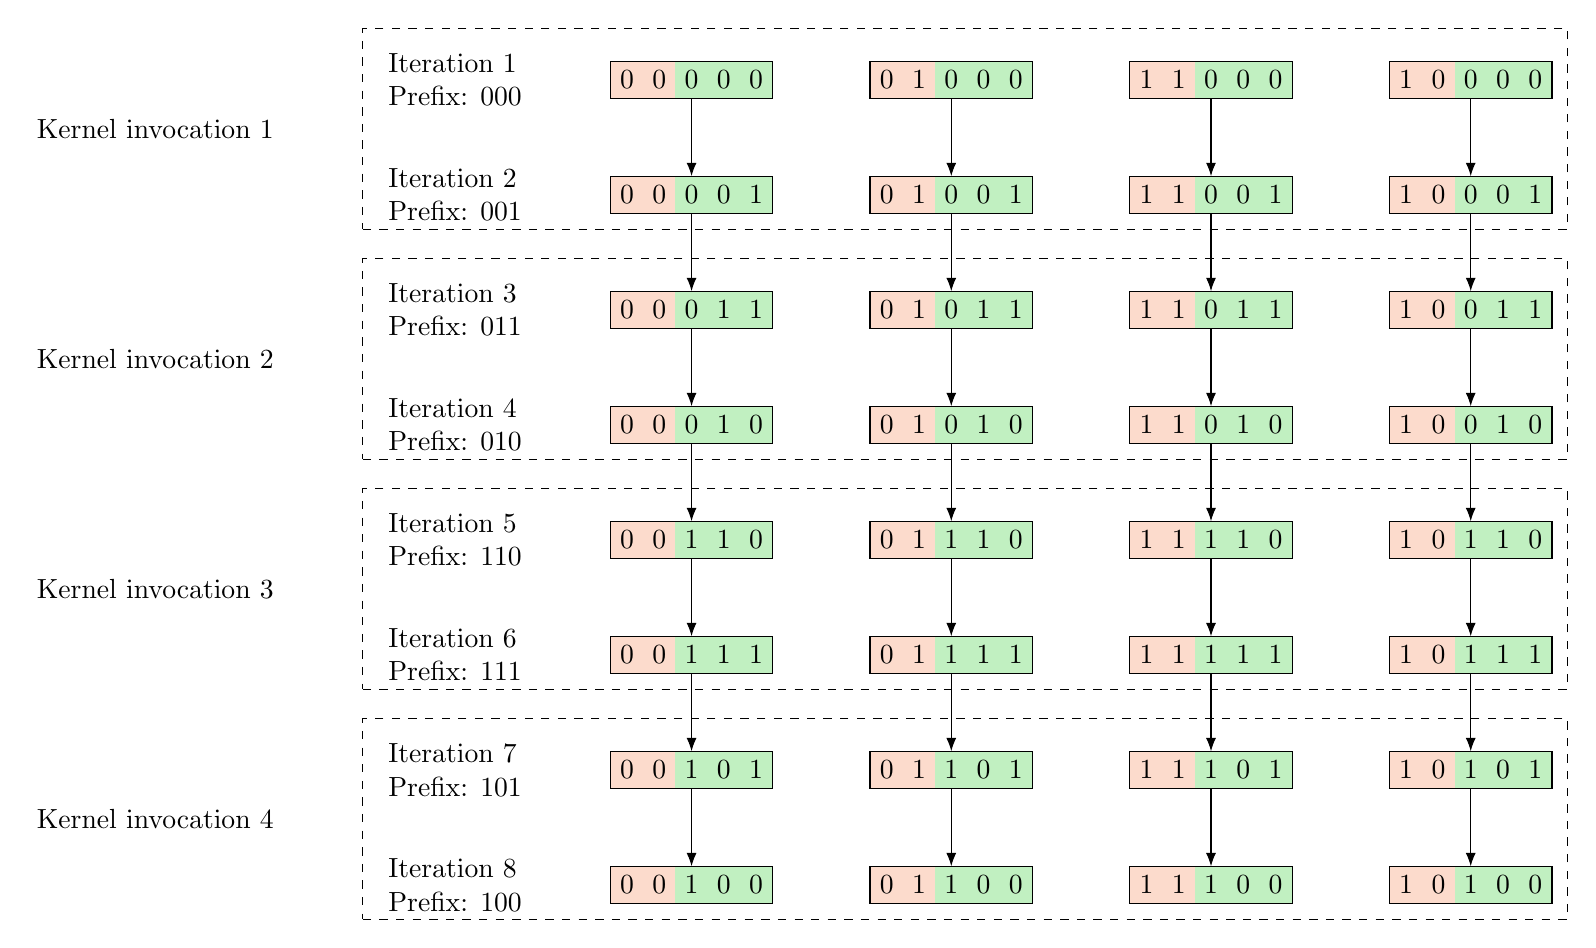
\begin{tikzpicture}[
    lane/.style={
        matrix of nodes,
        row sep=1cm,
        column 1/.style={nodes={fill=suffix}},
        column 2/.style={nodes={fill=suffix}},
        column 3/.style={nodes={fill=prefix}},
        column 4/.style={nodes={fill=prefix}},
        column 5/.style={nodes={fill=prefix}},
      }
  ]
  \matrix[lane]
  (suffix1)
  {
    0 & 0 & 0 & 0 & 0 \\
    0 & 0 & 0 & 0 & 1 \\
    0 & 0 & 0 & 1 & 1 \\
    0 & 0 & 0 & 1 & 0 \\
    0 & 0 & 1 & 1 & 0 \\
    0 & 0 & 1 & 1 & 1 \\
    0 & 0 & 1 & 0 & 1 \\
    0 & 0 & 1 & 0 & 0 \\
  };

  \matrix[lane, right=1cm of suffix1]
  (suffix2)
  {
    0 & 1 & 0 & 0 & 0 \\
    0 & 1 & 0 & 0 & 1 \\
    0 & 1 & 0 & 1 & 1 \\
    0 & 1 & 0 & 1 & 0 \\
    0 & 1 & 1 & 1 & 0 \\
    0 & 1 & 1 & 1 & 1 \\
    0 & 1 & 1 & 0 & 1 \\
    0 & 1 & 1 & 0 & 0 \\
  };

  \matrix[lane, right=1cm of suffix2]
  (suffix3)
  {
    1 & 1 & 0 & 0 & 0 \\
    1 & 1 & 0 & 0 & 1 \\
    1 & 1 & 0 & 1 & 1 \\
    1 & 1 & 0 & 1 & 0 \\
    1 & 1 & 1 & 1 & 0 \\
    1 & 1 & 1 & 1 & 1 \\
    1 & 1 & 1 & 0 & 1 \\
    1 & 1 & 1 & 0 & 0 \\
  };

  \matrix[lane, right=1cm of suffix3]
  (suffix4)
  {
    1 & 0 & 0 & 0 & 0 \\
    1 & 0 & 0 & 0 & 1 \\
    1 & 0 & 0 & 1 & 1 \\
    1 & 0 & 0 & 1 & 0 \\
    1 & 0 & 1 & 1 & 0 \\
    1 & 0 & 1 & 1 & 1 \\
    1 & 0 & 1 & 0 & 1 \\
    1 & 0 & 1 & 0 & 0 \\
  };

  \foreach \i in {1,2,3,4,5,6,7,8} {
      \foreach \j in {1,2,3,4} {
          \node [fit=(suffix\j-\i-1) (suffix\j-\i-5), draw=black, inner sep=0] {};
        }
    }
  \foreach \i in {1,2,3,4} {
      \foreach [count=\k] \j in {2,3,4,5,6,7,8} {
          \draw[-Latex] (suffix\i-\k-3) -- (suffix\i-\j-3);
        }
      }

  \node [left=1cm of suffix1-1-1, align=left]
  (label1)
  {Iteration 1 \\ Prefix: \pgfmathparse{\gray[0]}\pgfmathresult};

  \node [left=1cm of suffix1-2-1, align=left]
  (label2)
  {Iteration 2 \\ Prefix: \pgfmathparse{\gray[1]}\pgfmathresult};

  \node [left=1cm of suffix1-3-1, align=left]
  (label3)
  {Iteration 3 \\ Prefix: \pgfmathparse{\gray[2]}\pgfmathresult};

  \node [left=1cm of suffix1-4-1, align=left]
  (label4)
  {Iteration 4 \\ Prefix: \pgfmathparse{\gray[3]}\pgfmathresult};

  \node [left=1cm of suffix1-5-1, align=left]
  (label5)
  {Iteration 5 \\ Prefix: \pgfmathparse{\gray[4]}\pgfmathresult};

  \node [left=1cm of suffix1-6-1, align=left]
  (label6)
  {Iteration 6 \\ Prefix: \pgfmathparse{\gray[5]}\pgfmathresult};

  \node [left=1cm of suffix1-7-1, align=left]
  (label7)
  {Iteration 7 \\ Prefix: \pgfmathparse{\gray[6]}\pgfmathresult};

  \node [left=1cm of suffix1-8-1, align=left]
  (label8)
  {Iteration 8 \\ Prefix: \pgfmathparse{\gray[7]}\pgfmathresult};

  \node[fit=(label1) (suffix4-2-5), draw, dashed, inner sep = 0.2cm] (kernel1) {};
  \node[fit=(label3) (suffix4-4-5), draw, dashed, inner sep = 0.2cm] (kernel2) {};
  \node[fit=(label5) (suffix4-6-5), draw, dashed, inner sep = 0.2cm] (kernel3) {};
  \node[fit=(label7) (suffix4-8-5), draw, dashed, inner sep = 0.2cm] (kernel4) {};

  \node[left=1cm of kernel1] {Kernel invocation 1};
  \node[left=1cm of kernel2] {Kernel invocation 2};
  \node[left=1cm of kernel3] {Kernel invocation 3};
  \node[left=1cm of kernel4] {Kernel invocation 4};
\end{tikzpicture}

\end{document}
